\section{Python Problem - Wiener's LMS}\label{sec:p5}

\begin{enumerate}[(a)]
\item Figure \ref{fig:p5a} illustrates the prediction problem as an adaptive filter diagram, where the input is $x[n]$, the reference $d[n] = x[n+1] = \alpha x[n] + s[n] - 0.5 s[n-1]$, and the cost function $C(w) = \Expect{\abs{e[n]}^2} = \Expect{\abs{d[n] - y[n]}^2} = \Expect{\abs{d[n] - w^\top X[n]}^2}$.
\begin{figure}[htbp]
	\centering
	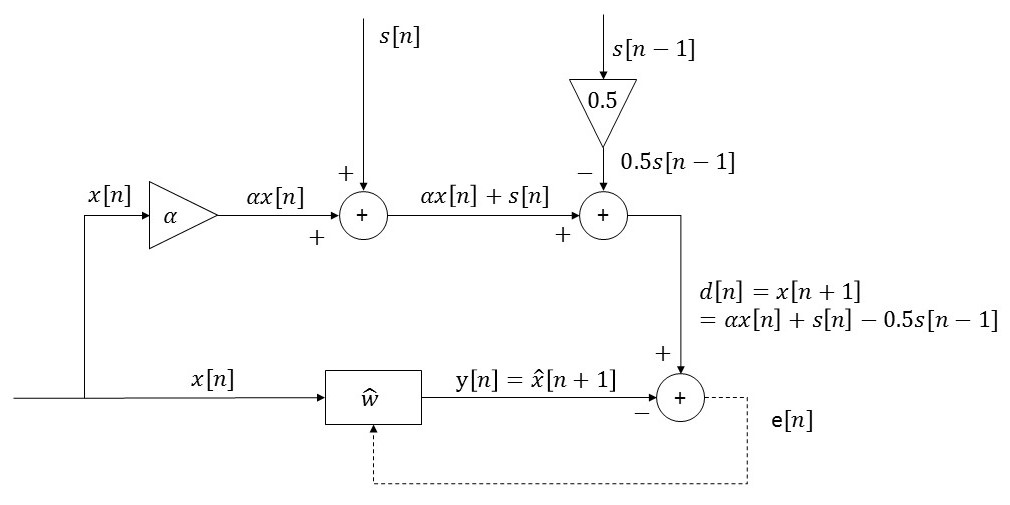
\includegraphics[width=\textwidth]{images/p5a}
	\caption{Adaptive filter diagram}
	\label{fig:p5a}
\end{figure}

\item 
We have \[x[n+1] = \alpha x[n] + s[n] - 0.5 s[n-1]\] Therefore, its Z-transform is
\begin{align*}
	X(z)z &= \alpha X(z) + S(z) -0.5 S(z) z^{-1} \\
	\Leftrightarrow X(z)(z-\alpha) &= S(z) \frac{1 - 0.5 z^{-1}}{z - \alpha} \\
	\Rightarrow H(z) &= \frac{1 - 0.5 z^{-1}}{z - \alpha}
\end{align*}
Since $A_s(z) = 1$,
\begin{align*}
	A_x(z)
	&= H(z)H(z^{-1}) \\
	&= \frac{1 - 0.5 z^{-1}}{z - \alpha} \frac{1 - 0.5 z}{z^{-1} - \alpha} \\
	&= \frac{0.5z - 1.25 +0.5z^{-1}}{\alpha z - (1+\alpha^2) +\alpha z^{-1}} \\
	&= \frac{0.5z^2 - 1.25z +0.5}{\alpha z^2 - (1+\alpha^2)z +\alpha} \\
	\Rightarrow a_x[n]
	&= \frac{0.25(2\alpha^2 - 5\alpha +2)(\alpha^{2n}-1)\alpha^{-n-1}(1-\theta(-n))}{\alpha^2 - 1} + \frac{0.5\theta(-n)}{\alpha}
\end{align*}
where $\theta(n)$ is the Heaviside step function. Therefore
\[a_x[n] = \begin{cases}
\frac{0.5}{\alpha} & n \leq 0 \\
\frac{0.5((\alpha-2.5)\alpha+1)\alpha^{-n-1}(\alpha^{2n}-1)}{\alpha^2 - 1} & \text{else}
\end{cases}\]

\end{enumerate}